% !TEX TS-program = xelatex
\documentclass[12pt,letterpaper]{article}

% ===========================
% BASIC PACKAGES
% ===========================
\usepackage[british]{babel}
\usepackage[final]{microtype}
\usepackage{amsmath,amssymb}
\numberwithin{equation}{section}
\usepackage{graphicx}
\usepackage{booktabs}
\usepackage{tabularx}
\usepackage{array}
\usepackage{float}
\usepackage{xspace}
\usepackage{tikz}
\usetikzlibrary{calc,positioning,arrows.meta,fit,backgrounds,shapes.geometric}
\usepackage{fontspec}
\setmainfont{EB Garamond}[Numbers=OldStyle,Ligatures=TeX]
\newfontfamily\ipafont{Charis SIL}
\newcommand{\ipa}[1]{{\ipafont #1}}
\providecommand{\liningnums}[1]{{\addfontfeatures{Numbers=Lining}#1}}
\setmonofont{Inconsolata}[Scale=MatchLowercase]

% ===========================
% PAGE LAYOUT
% ===========================
\usepackage[
  letterpaper,
  inner=1.25in,
  outer=1in,
  top=1in,
  bottom=1.25in,
  marginparwidth=0.6in,
]{geometry}

% ===========================
% HEADINGS
% ===========================
\usepackage{titlesec}
\titleformat{\section}{\normalfont\scshape}{\llap{\thesection\quad}}{0pt}{}
\titleformat{\subsection}{\normalfont\scshape}{\thesubsection\quad}{0pt}{}
\titleformat{\subsubsection}{\normalfont}{\thesubsubsection\quad}{0pt}{}
\titleformat{\paragraph}[runin]{\normalfont\scshape}{\theparagraph}{1em}{}
\titlespacing*{\section}{0pt}{2ex plus 1ex minus .2ex}{1ex plus .2ex}
\titlespacing*{\subsection}{0pt}{1.5ex plus 1ex minus .2ex}{0.5ex plus .2ex}
\titlespacing*{\subsubsection}{0pt}{1ex plus 0.5ex minus .1ex}{0.3ex plus .1ex}
\titlespacing*{\paragraph}{0pt}{1ex plus 0.5ex minus .1ex}{1em}

% ===========================
% RUNNING HEADS
% ===========================
\usepackage{fancyhdr}
\pagestyle{fancy}
\fancyhf{}
\fancyhead[L]{\small\scshape\leftmark}
\fancyhead[R]{\small\thepage}
\setlength{\headheight}{26pt}
\addtolength{\topmargin}{-12.4pt}
\renewcommand{\headrulewidth}{0pt}

% ===========================
% COLOURS & HYPERLINKS
% ===========================
\usepackage{xcolor}
\definecolor{linkmaroon}{RGB}{128,0,32}
\usepackage{hyperref}
\hypersetup{
  colorlinks=true,
  linkcolor=linkmaroon,
  citecolor=linkmaroon,
  urlcolor=linkmaroon,
  pdftitle={Grammaticality de-idealized: An etiological account},
  pdfauthor={Brett Reynolds},
}

% ===========================
% QUOTATIONS
% ===========================
\usepackage[style=british]{csquotes}

% ===========================
% SEMANTIC MACROS
% ===========================
\newcommand{\term}[1]{\textsc{#1}}
\newcommand{\mention}[1]{\textit{#1}}
\newcommand{\mentionh}[1]{⟨#1⟩}
\newcommand{\olang}[1]{\textit{#1}}
\newcommand{\abbr}[1]{\textsc{#1}}
\newcommand{\eg}{e.g.\,\xspace}
\newcommand{\ie}{i.e.\,\xspace}

% ===========================
% JUDGEMENT MARKERS (TEXT-MODE SAFE)
% ===========================
\newcommand{\judgesep}{\kern-0.15em}
\newcommand{\ungram}[1]{*\judgesep#1}
\newcommand{\marg}[1]{?\judgesep#1}
\newcommand{\odd}[1]{\#\judgesep#1}

% ===========================
% LINGUISTIC EXAMPLES
% ===========================
\usepackage{langsci-gb4e}
\makeatletter
\@ifundefined{noautomath}{}{\noautomath}
\makeatother

% ===========================
% BIBLIOGRAPHY
% ===========================
\usepackage[backend=biber,style=apa,natbib=true,doi=true,isbn=false,url=true]{biblatex}
\addbibresource{refs.bib}
\newcommand{\posscite}[1]{\citeauthor{#1}'s (\citeyear{#1})}
\usepackage{orcidlink}

% ===========================
% TITLE
% ===========================
\title{Grammaticality de-idealized:\\An etiological account of stable repertoire exclusion}
\author{Brett Reynolds \orcidlink{0000-0003-0073-7195}\\Humber Polytechnic \& University of Toronto\\\href{mailto:brett.reynolds@humber.ca}{brett.reynolds@humber.ca}}
\date{}

\begin{document}
\maketitle

\begin{abstract}
The constitutive account of grammaticality explains what grammatical status \emph{is}; this companion paper asks the etiological question: why do repertoire-status trajectories settle where they do? Two complementary modules are developed. \term{Opportunity-sensitive preemption} explains how learners infer exclusion from systematic absence in niches where competitors succeed; the evidential strength of absence scales with opportunity-set size. \term{Coordination equilibria} explain why exclusions persist: once an equilibrium excludes a form, deviation is penalized and expectations crystallize. These modules interact with \term{stochastic drift}, which can move rare forms in either direction independently of systematic pressures. Entry into the repertoire faces higher thresholds than exit~-- a principled asymmetry grounded in evidence, coordination, learning, and social-norm considerations. The modules yield a typology of stability profiles: gaps sustained by both modules are maximally stable; gaps sustained by one module drift under appropriate manipulations; gaps sustained by neither may exit by chance. Domain-specific equilibria explain stable variation: competing forms persist when different registers occupy different coordination equilibria. The framework makes testable predictions, specifies fragility conditions for destabilization, and explains categorical behaviour without treating categoriality as a primitive.
\end{abstract}

\noindent Keywords: grammaticality; repertoire exclusion; preemption; coordination equilibrium; conditioned stability; etiology

\section{Introduction}

Some grammatical exclusions feel utterly categorical. \mention{*Which did you buy car?} isn't marginal or awkward; it's \emph{out}~-- categorically excluded from the English repertoire, impervious to context, register, or goodwill. Other exclusions drift: split infinitives were once policed sharply and are now unremarkable in many contexts. Still others never stabilize: gradient, variable, speaker-dependent.

What explains these differences? Knowing what grammaticality \emph{is}~-- what makes a form grammatical or not~-- doesn't automatically answer this question. Even if we know that grammaticality depends partly on whether a form is in the community's repertoire, we still need to explain \emph{why} some forms get excluded from that repertoire and stay excluded, while others drift in or out over time.

This paper develops an \term{etiological account}: an explanation of why repertoire exclusions arise and persist. The account has two modules:

\begin{enumerate}
  \item \textbf{Opportunity-sensitive preemption.} Learners infer that a form is excluded from the repertoire when it systematically fails to appear in contexts where competitors reliably succeed. The evidential strength of absence depends on the size of the opportunity set: zero tokens out of five opportunities tells us little; zero tokens out of five thousand is decisive.
  \item \textbf{Coordination equilibria.} Once a form is excluded, the exclusion is maintained by the self-reinforcing logic of coordination. Speakers expect the form to be out; hearers interpret deviation as error; deviant speakers bear the cost. Even if preemption pressure were somehow removed, mutual expectations would maintain exclusion.
\end{enumerate}

The two modules are complementary, not competing. Preemption explains how forms get \emph{driven out} of the repertoire; coordination explains why they \emph{stay out}. A form can be excluded by strong preemption alone, by strong coordination alone, or by both. The combination determines the stability profile: gaps sustained by both modules are maximally stable; gaps sustained by only one module drift under the right conditions; gaps sustained by neither never fully categoricalize.

The two modules can be read as analytically separable mechanisms in one coupled system: learners infer repertoire status from distributional opportunity patterns, and communities maintain (and signal) repertoire boundaries through coordination pressures whose penalties are themselves publicly observable. Supply~-- the injection of tokens for forms not yet mutually expected~-- is not a third module but the positive-evidence channel in the same evidential dynamics that underwrite preemption; whether that evidence is amplified into invasion is jointly shaped by coordination equilibria and the supply conditions themselves, with drift as the finite-sampling noise in both directions.

This approach has three payoffs. First, it explains categorical behaviour without treating categoriality as a primitive. Categorical constraints emerge from the dynamics of preemption and coordination, not from built-in structural bans. Second, it yields testable predictions about how exclusions behave under manipulation~-- predictions that distinguish gaps sustained by both modules from those sustained by only one. Third, it connects grammatical structure to broader theories of convention, norm enforcement, and cultural evolution, positioning grammar within the ecology of socially sustained regularities.

\S\ref{sec:distinction} introduces the constitutive-etiological distinction and the formal framework. \S\ref{sec:preemption} develops Module~1 (preemption). \S\ref{sec:coordination} develops Module~2 (coordination equilibria). \S\ref{sec:integration} integrates the two modules and derives stability profiles. \S\ref{sec:predictions} states empirical predictions and disconfirmation conditions. \S\ref{sec:conclusion} concludes.

\section{The constitutive--etiological distinction}\label{sec:distinction}

A constitutive account says what a thing \emph{is}. An etiological account says why it came to be and why it stays that way. The two are logically independent: knowing that water is H$_2$O tells us nothing about why this lake has water in it. Knowing what grammaticality is~-- how it decomposes into structural, semantic, and social components~-- tells us nothing about why particular forms end up excluded or included.

This paper develops an etiological account of repertoire exclusion. Its target is a single question: given that a form is structurally parseable and semantically coherent, why does the community sometimes treat it as categorically excluded from the repertoire?

\subsection{The constitutive framework in brief}

Why do some utterances strike us as ungrammatical? The constitutive account starts from the observation that utterances can fail at different levels~-- and the level of failure matters for explanation.

\paragraph{Three sources of failure.} Consider three utterances:
\begin{exe}
  \ex\label{ex:map-fail} \ungram{The of into slept.}
  \ex\label{ex:k-fail} \odd{Colourless green ideas sleep furiously.}
  \ex\label{ex:ct-fail} \ungram{I have 25 years.} (intended: stating one's age in English)
\end{exe}

(\ref{ex:map-fail}) fails because no parse assigns it a coherent structure-value pairing: it doesn't \emph{map}. (\ref{ex:k-fail}) parses fine but fails because the values clash: colourless things aren't green, abstract entities don't sleep. It lacks \term{interpretive coherence}. (\ref{ex:ct-fail}) is different: the structure is trivial, the meaning is transparent, and yet English speakers reject it. What's wrong isn't the form itself but its \term{repertoire status}: this isn't how English speakers express age, even though French and Spanish speakers use an analogous construction without difficulty.

The constitutive account captures these distinctions by decomposing grammatical status into three quantities:

\begin{enumerate}
  \item $\mathsf{map}(u,c)$: \term{mapping viability}. Does the form support a systematic pairing of structure and value? This includes successful parsing, morphological well-formedness, and the availability of a compositional interpretation. If parsing fails outright or no coherent structure-value mapping exists, $\mathsf{map}$ is zero or near-zero. Example~(\ref{ex:map-fail}) fails here.

  \item $K(u,c)$: \term{interpretive coherence}. Do the values carried by the form cohere with one another and with the conditioning state? Semantic anomaly (\ref{ex:k-fail}), pragmatic incongruity (answering a yes/no question with an existential claim), and logical incoherence (presupposition failure) all lower $K$. A form can map perfectly but fail to cohere.

  \item $C_t(u,c)$: \term{repertoire status}. Is the form part of the community's grammatical repertoire for conditioning state $c$ at time $t$? This is the socially contingent component: it can vary across dialects, registers, and eras without any change in $\mathsf{map}$ or $K$. Example~(\ref{ex:ct-fail}) fails here: the form maps, it coheres, but English speakers don't use it for this purpose.
\end{enumerate}

\paragraph{Conditioning states.} The subscript $c$ in these quantities denotes the \term{conditioning state}: the full context that determines what counts as grammatical \emph{here and now}. This includes the register (formal vs.\ casual), the speech community (which dialect?), the genre (academic prose vs.\ text message), the discourse context (what's been said so far), and the communicative intentions in play. The same form can have different status across conditioning states: a contraction acceptable in casual speech may be excluded from formal writing; a dialectal construction in-repertoire for one community may be excluded for another. Grammaticality is always \emph{conditioned}.

\paragraph{Why multiplication?} The three quantities combine multiplicatively:
\begin{equation}\label{eq:stability}
\widetilde{G}_t(u,c) = \mathsf{map}(u,c) \cdot K(u,c) \cdot C_t(u,c).
\end{equation}
The product structure captures the intuition that any zero kills the result. A form that doesn't parse ($\mathsf{map} = 0$) can't be rescued by being in the repertoire. A form that's categorically excluded ($C_t = 0$) can't be rescued by perfect coherence. The quantities are individually necessary: failure at any level is sufficient for ungrammaticality.

This gives us a continuous \term{stability score} $\widetilde{G}_t(u,c)$ that ranges from zero (any component is zero) to values approaching one (all components are high). But grammaticality judgments are often categorical: speakers say \enquote{yes} or \enquote{no}, not \enquote{0.73}. How does a continuous score yield categorical judgments?

\paragraph{The threshold.} Categorical membership emerges by thresholding:
\begin{equation}\label{eq:membership}
G_t(u,c) = \mathbb{I}\!\left[\widetilde{G}_t(u,c) \ge \tau(c)\right],
\end{equation}
where $\mathbb{I}[\cdot]$ is the indicator function (1 if the condition holds, 0 otherwise) and $\tau(c)$ is a situation-sensitive \term{threshold}. When the stability score clears the threshold, the form counts as grammatical in that conditioning state; when it falls short, it counts as ungrammatical.

What determines $\tau(c)$? The threshold reflects coordination stakes. In high-stakes communicative situations~-- formal presentations, institutional gatekeeping, contexts where misunderstanding has serious consequences~-- the cost of coordination failure is high, and so is $\tau$. Speakers police their output more carefully; hearers are less tolerant of deviation. In low-stakes situations~-- casual in-group conversation, play, contexts where repair is cheap~-- $\tau$ drops. The same form with the same $\widetilde{G}$ may clear the threshold in one context and fail in another. This is why register matters: it shifts the threshold, not (necessarily) the underlying stability score.

\subsection{This paper's focus: $C_t$ trajectories}

Everything above is \emph{constitutive}. It specifies what grammatical status is, not what produces it. This paper is concerned entirely with $C_t$~-- the repertoire-status component~-- and with three etiological questions about it.

\paragraph{What $C_t$ is.} $C_t(u,c)$ is a community-level variable: the probability that a randomly sampled competent community member will treat $u$ as licensed in conditioning state $c$. This is an \emph{epistemic} characterisation~-- it describes the distribution of internal grammar-states or licensing beliefs across the population. But $C_t$ is also observable \emph{behaviourally}: it manifests as the population frequency with which $u$ is produced (or accepted without repair) for a given communicative job under conditioning state $c$. The two characterisations are linked by the assumption that production and acceptance behaviour reliably track internal licensing states, at least in aggregate. Module~1 below provides a microfoundation for how individual beliefs about licensing collapse toward zero under preemption. Module~2 provides a microfoundation for how social responses (correction, repair, sanction) make those beliefs stable and mutually reinforcing. The two modules target different levels of analysis but converge on the same community-level outcome.

\paragraph{Proximate channels.} Both modules require proximate mechanisms that translate population-level states into individual behaviour. In humans, one such channel is the \term{feeling of ungrammaticality} $F$~-- the subjective signal that a form is anomalous. Preemption accumulates partly because forms lacking positive evidence feel increasingly odd; coordination equilibria are maintained partly because deviation triggers negative affect that prompts correction or sanction.

But $F$ is not the only proximate channel, and making it indispensable would be a mistake. The etiological story should be robust to variation in introspective access, metalinguistic ideology, and affective response. Other channels include: conditioned avoidance (behavioural inhibition without conscious affect), predictive-processing surprisal (elevated prediction error that slows production/comprehension), and reputational inference (attributing incompetence or outsider status to deviants). All of these can implement the penalty structure that Module~2 requires, and all can feed into the avoidance behaviour that generates the opportunity patterns Module~1 exploits.

The explanatory target is therefore not \enquote{what produces the feeling of ungrammaticality} but \enquote{what stabilizes the penalty/payoff structure that excludes a form from the repertoire}. $F$ is one human-typical implementation of that structure; the structure itself is what the modules explain.

\paragraph{Question 1: How does $C_t$ get driven toward zero?} Consider the utterance \mention{I have 25~years} intended to state the speaker's age. English speakers reject this form: $C_t$ is near zero for this conditioning state (age-stating in English). Yet the form is parseable ($\mathsf{map} > 0$) and coherent ($K > 0$)~-- Spanish, French, and many other languages use an analogous construction without difficulty. What mechanism drives $C_t$ toward zero for structurally viable, semantically coherent forms?

\paragraph{Question 2: Why does $C_t$ stay near zero?} Once $C_t$ has crashed, why does it stay low? Individual speakers encounter new usage constantly; communities change. Yet many exclusions persist for centuries. What sustains them?

\paragraph{Question 3: What predicts drift versus stability?} Some exclusions are maximally stable: left-branch extraction in English (\ungram{Which did you buy car?}) has been categorically excluded for as long as the construction has been documentable. Others drift: split infinitives were once sharply policed and are now unremarkable in many registers. What distinguishes stable gaps from drifting ones?

\subsection{Two complementary modules}

The remainder of this paper develops two explanatory modules, each targeting a different aspect of the etiological question.

\term{Module~1: Opportunity-sensitive preemption} (\S\ref{sec:preemption}) explains how $C_t$ gets driven toward zero. The mechanism is Bayesian learning under informative opportunity sets. When a form faces strong competitors that reliably win in well-attested niches, the learner accumulates strong negative evidence; $C_t$ crashes. When the opportunity set is sparse or the competitors are weak, $C_t$ drifts slowly and may never reach categorical exclusion.

\term{Module~2: Coordination equilibria} (\S\ref{sec:coordination}) explains why $C_t$ stays near zero once it gets there. The mechanism is game-theoretic: communicative situations are coordination games with multiple equilibria, and once an equilibrium excludes a form, unilateral deviation is penalized. Even if preemption pressure were somehow removed, the coordination equilibrium would maintain exclusion because mutual expectations have crystallized.

The two modules make independent predictions. A form can be excluded by strong preemption alone, by coordination pressure alone, or by both. The integration (\S\ref{sec:integration}) shows how the combination predicts which gaps are maximally stable (both modules), which drift when conditions shift (one module), and which never fully stabilize (neither module dominant).

\section{Module 1: Opportunity-sensitive preemption}\label{sec:preemption}

The first module addresses Question~1: how does $C_t$ get driven toward zero for forms that are structurally viable and semantically coherent? The answer invokes \term{statistical preemption}~-- the mechanism by which learners infer that a form is excluded from the repertoire on the basis of its systematic absence where competitors succeed \citep{goldberg2019, Goldberg2011}. But preemption strength isn't uniform across constructions. It depends critically on \emph{how much opportunity} the form has had to appear.

\subsection{Niches, competitors, and opportunity sets}\label{sec:niches}

Define a \term{constructional niche} $n$ as a communicative job: a recurrent communicative intention that speakers routinely encode grammatically. \enquote{State a person's age}, \enquote{question a proposition}, \enquote{request information about a location}, and \enquote{express completed action} are all niches. A niche is specified independently of the forms that realize it~-- it's the slot in communicative ecology that forms compete to fill.

For any niche $n$ in conditioning state $c$, define the \term{competitor set} $V_{n,c}$ as the set of grammatical variants that can realize $n$ in $c$. The conditioning state matters: competitors available in casual speech may differ from those available in formal writing. The age-stating niche in colloquial English has competitors including \mention{I'm 25}, \mention{I'm 25 years old}, and \mention{I'm 25 years of age}. The question niche has competitors including fronted interrogative phrases (\mention{What did you buy?}) and in-situ interrogative phrases (\mention{You bought what?}), though the latter is pragmatically restricted.

\paragraph{Opportunity as counterfactual suitability.} A competitor token counts as an opportunity for the target form only when the target would have achieved equal niche-satisfaction at comparable cost in that same conditioning state. Not every use of a competitor is a context where the target was in the choice set: information-structural requirements, register constraints, or pragmatic preconditions may rule it out. A raw count of competitor tokens therefore overstates the opportunity mass.

The cleanest formalization treats opportunity as \emph{weighted}. Let $w_i \in [0,1]$ be the counterfactual suitability of the target $u$ in the $i$th competitor-token context~-- the degree to which $u$ would have served equally well. The \term{effective opportunity count} is then:
\begin{equation}\label{eq:opportunity}
N^{\ast}_t(n,c) = \sum_{i=1}^{|\text{competitor tokens}|} w_i.
\end{equation}
When $w_i = 1$ for all tokens (full substitutability), this reduces to the raw count. In practice, the weights are rarely known precisely, but the conceptual move is important: it makes explicit that absence is evidential only relative to \emph{effective} opportunity, not raw frequency.

\paragraph{Operationalising $w_i$: separating context-eligibility from licensing.} The opportunity weights $w_i$ are meant to track whether the $i$th competitor-token context is one in which the target \emph{would have been in the choice set} \emph{if it were licensed}. Estimating $w_i$ by asking speakers whether the excluded target is \enquote{natural} risks circularity: such judgments largely recover $C_t$ rather than context-eligibility.

A more conservative operationalisation therefore targets eligibility constraints using only contrasts among already-licensed variants. In niches where alternations are pragmatically restricted (e.g.\ interrogative in-situ versus interrogative fronting), one can estimate an eligibility region by modelling the distribution of attested variants over discourse features (echo status, focus marking, register, information-structural configuration). A competitor token then counts as an opportunity for the target to the degree that its context falls inside that eligibility region: $w_i$ is high when the context matches the estimated preconditions and low otherwise. In broad niches with near-free alternation among licensed variants (e.g.\ copular age-stating variants), eligibility constraints are weak and $w_i$ will be close to $1$ for most competitor tokens.

This yields an $N^{\ast}$ proxy that is sensitive to pragmatic and register constraints without consulting acceptability of the target form itself.

\paragraph{A concrete pipeline.} To make this operational: (i) define a feature set over competitor contexts (discourse status, information structure, register markers, clause type); (ii) fit a model predicting variant choice among the licensed alternants; (iii) identify the high-density region of the feature space where near-free alternation holds~-- this is the eligibility region; (iv) for each competitor token, compute its distance to that region and set $w_i$ accordingly (high inside, decaying outside). The resulting $N^{\ast}$ is a sum of fractional pseudo-counts rather than raw tokens. No claim is made that this is easy; the point is that the method is specifiable in principle, using only data from licensed variants, and avoids the circularity of asking about the excluded target directly.

\paragraph{Absence is evidential only relative to effective opportunity.} Zero tokens of a form tells us almost nothing in isolation. Zero tokens out of five effective opportunities leaves massive uncertainty~-- the form might simply not have been needed. Zero tokens out of five thousand effective opportunities, where competitors have won every time, provides strong evidence that the form is excluded.

This is the key insight: \emph{categorical exclusion} ($C_t \approx 0$) requires not just absence of positive evidence but presence of \emph{informative} negative evidence. The informativeness of absence is determined by the effective opportunity count, not by raw competitor frequency.

\paragraph{Worked example: age-stating.} Reynolds (in prep.) develops this example in detail. The niche is \enquote{state a person's age in response to direct or indirect enquiry}. In spoken British English corpora, the copular competitors rack up thousands of tokens per million words~-- $N^{\ast}$ is large. The have-construction (\mention{I have 25 years}) has zero tokens. Given the massive opportunity set, that zero is probative: it licenses the inference that the construction is categorically excluded for English speakers, even though it's perfectly grammatical in French (\mention{J'ai 25 ans}) and Spanish (\mention{Tengo 25 años}).

\subsection{Preemption strength as a function of opportunity-set robustness}\label{sec:preemption-strength}

The intuition above can be formalized in a Bayesian learning framework. Let $\theta_u$ be the latent probability that form $u$ is licensed for niche $n$ in conditioning state $c$. The learner starts with a prior $\theta_u \sim \text{Beta}(\alpha_0, \beta_0)$~-- agnostic, perhaps, with $\alpha_0 = \beta_0 = 1$.

Evidence updates the posterior. Positive evidence (hearing $u$ in niche $n$) increments $\alpha$. Negative evidence~-- hearing a competitor $v \ne u$ when $u$ could have served~-- increments $\beta$. After observing $s_t$ successes (tokens of $u$) and $f_t$ failures (tokens of competitors) in niche $n$, the posterior is:
\begin{equation}\label{eq:beta-update}
\theta_u \mid \text{data} \sim \text{Beta}(\alpha_0 + s_t, \beta_0 + f_t).
\end{equation}
The posterior mean $\hat{\theta}_u = (\alpha_0 + s_t)/(\alpha_0 + \beta_0 + s_t + f_t)$ serves as an estimate of licensing status. If $s_t = 0$ and $f_t$ is large, the posterior crashes toward zero. This is the Bayesian reconstruction of preemption: the absence of $u$ combined with the presence of competitors provides evidence for exclusion, and the strength of that evidence scales with $f_t$~-- the effective opportunity count.

\paragraph{A note on what learners observe.} Learners don't observe literal Bernoulli trials where the target is attempted and fails; they observe production choices generated by speakers with their own grammars, pragmatic constraints, and processing limitations. The inference from \enquote{competitors won} to \enquote{target is unlicensed} is justified only under assumptions about niche equivalence (the competitor and target could have served the same communicative function) and speaker rationality (speakers don't systematically avoid licensed forms). These assumptions are implicit in all preemption-based accounts \citep[cf.][]{Goldberg2011, goldberg2019}; making them explicit clarifies why high-opportunity niches are special. In high-opportunity niches, stable production preferences generate sharper inferences because pragmatic and processing noise averages out across many observations.

\paragraph{Preemption mass and the Bayesian link.} The effective opportunity count $N^{\ast}_t$ from \eqref{eq:opportunity} serves directly as the measure of preemption pressure: it is the cumulative weighted competitor evidence that drives the posterior toward zero. Because the $w_i$ weights can be fractional, $N^{\ast}_t$ functions as a sum of pseudo-counts rather than literal trial counts. Large $N^{\ast}_t$ means strong preemption pressure: many effective opportunities where $u$ could have appeared but a competitor won instead. Small $N^{\ast}_t$ means weak pressure: not enough competitor evidence to drive the posterior toward zero decisively.

\paragraph{Two trajectories.} Consider two forms, both with zero positive tokens ($s_t = 0$):

\begin{itemize}
  \item \textbf{High-opportunity niche:} The form faces thousands of competitor tokens annually. $N^{\ast}_t$ is massive, the posterior crashes to near-zero early in acquisition, and $C_t$ stabilizes near zero. This is the profile of categorical exclusion.
  \item \textbf{Low-opportunity niche:} The form faces only a handful of competitor tokens. $N^{\ast}_t$ remains small, the posterior drifts slowly, and $C_t$ may settle at an intermediate value~-- uncertain, gradient, variable across speakers. This is the profile of a rare construction, not a categorical gap.
\end{itemize}

The distinction matters empirically. Constructions treated as \enquote{categorical} by linguists should show large $N^{\ast}$ via high competitor counts; constructions treated as \enquote{rare} or \enquote{uncertain} should show small $N^{\ast}$. If the correlation fails~-- if constructions widely judged as categorical lack robust opportunity proxies~-- then the preemption mechanism is not the explanation for their status.

\paragraph{Connection to operator contrasts.} Not all grammatical contrasts are equal. It helps to distinguish three levels:

\begin{itemize}
  \item \textbf{Expression-shape:} Basic word-level well-formedness. \mention{*Goed} for \mention{went} violates expression-shape~-- it's not a word of English.
  \item \textbf{Operators:} Grammatical contrasts that configure the speech act, allocate participant roles, and constrain uptake. Clause-typing (declarative vs.\ interrogative vs.\ imperative), argument linking (subject vs.\ object), and tense/aspect marking are operators. They structure how the utterance functions in discourse.
  \item \textbf{Payload:} The semantic and pragmatic content carried by lexical choices and compositional meaning. Word choice, collocational preferences, and stylistic register are payload-level.
\end{itemize}

Operators tend to inhabit high-frequency niches: clause-typing and argument linking are needed in every clause. This predicts that operator violations face maximal preemption pressure: the opportunity sets are enormous, competitors win reliably, and $C_t$ crashes to near-zero for any form that doesn't conform to the operator paradigm. Payload mismatches, by contrast, face weaker preemption because the niches are more varied and substitutability is higher.

\subsection{Niche variation and register effects}\label{sec:niche-variation}

Because $C_t$ is conditioned on $c$, the same form can face different preemption pressure across conditioning states. A form excluded in one register may survive in another simply because the opportunity set differs.

\paragraph{Dialectal forms.} Consider \mention{I might could help you}~-- the double-modal construction found in some Southern US and Scottish dialects. For speakers of these dialects, the construction is in the repertoire; $C_t > 0$ for the relevant conditioning states (tentative offers, hedged permissions). For speakers outside these dialects, it's excluded: $C_t \approx 0$. The difference isn't structural~-- both groups parse the utterance~-- but social: the two speech communities have different coordination equilibria (Module~2), and for the excluding community, competitor realizations (single modals, epistemic adverbs) have won reliably enough that preemption has crashed $C_t$.

\paragraph{Register-sensitivity.} Some gaps appear categorical in formal registers but relax in informal ones. The explanation may involve both modules: (i) formal registers have higher $\tau(c)$ thresholds, so even moderate $C_t$ doesn't clear the bar, and (ii) the opportunity sets differ~-- certain competitors dominate in formal writing but are absent in casual speech, weakening preemption pressure.

\subsection{Interaction with processing difficulty}\label{sec:processing}

Preemption isn't the whole story. Some forms are excluded not (or not only) because competitors have won, but because processing them is difficult. Processing costs can compound preemption, pushing $C_t$ even lower, but the two mechanisms are separable.

\paragraph{Processing costs without exclusion.} Centre-embedded relative clauses (\mention{The rat the cat the dog chased bit died}) are notoriously difficult to process. Yet they're not categorically excluded from the repertoire: speakers judge them grammatical once they work through the parse, and careful speakers occasionally produce them in registers that tolerate complexity. High processing cost slows acquisition and reduces frequency, but it doesn't zero out $C_t$.

\paragraph{Preemption without processing costs.} The age-stating example (\mention{I have 25 years}) involves no processing difficulty~-- the structure is trivial and the meaning is transparent. What excludes it is pure preemption: copular competitors have won every opportunity, and the posterior has crashed.

\paragraph{Double exclusion.} Left-branch extraction (\ungram{Which did you buy car?}) faces both pressures. The form is difficult to parse because it separates the determiner from its noun~-- a dependency that English otherwise disallows and that hearers don't expect. The parser encounters \mention{Which did you buy}, which looks like a complete constituent question; the stranded \mention{car} then forces costly reanalysis. But LBE also faces massive preemption: the interrogative-fronting competitor (\mention{Which car did you buy?}) wins reliably in an enormous opportunity set. The combination produces maximally sharp exclusion~-- the phenomenon feels \enquote{more ungrammatical} than either processing difficulty or preemption alone would predict.

\paragraph{Where processing costs live.} Processing costs arise from two sources: structural properties of the form (garden-path potential, center-embedding, working memory load) and expectation-based difficulty (forms with low $C_t$ are less predicted, less primed, harder to integrate). The constitutive account has to make an explicit commitment about how these costs enter the stability score. Two options are defensible:

\begin{enumerate}
  \item Processing costs lower $\mathsf{map}(u,c)$, on the grounds that reliable real-time parsing is part of mapping viability in actual use. A form that systematically triggers garden-path reanalysis has degraded mapping viability even if an offline parse is available.
  \item Processing costs constitute an independent multiplicative factor $P(u,c)$, yielding $\widetilde{G} = \mathsf{map} \cdot K \cdot C_t \cdot P$. This separates structural well-formedness from real-time feasibility.
\end{enumerate}

For present purposes, I adopt option (i): processing costs lower $\mathsf{map}$. This keeps the constitutive architecture minimal (three factors, not four) and captures the intuition that a form which can't be reliably parsed in real time doesn't fully \enquote{map} in the relevant sense. The product rule then predicts that forms with low $\mathsf{map}$ (processing difficulty) and low $C_t$ (preemption) compound multiplicatively. LBE is doubly sustained in the etiological sense (strong preemption + strong coordination, as defined in \S\ref{sec:integration}), and \emph{additionally} degraded at the $\mathsf{map}$ level by processing costs~-- triply buttressed, as it were. The multiplicative architecture means these sources of exclusion don't merely add; they compound.

\subsection{Entry as positive evidence: supply inside the same dynamics}\label{sec:arise}

The Bayesian update in \eqref{eq:beta-update} is already bidirectional. Preemption was foregrounded because it explains a striking fact about exit: $C_t$ can be driven toward zero even when the learner never hears the target, provided the learner repeatedly observes competitors in contexts that count as effective opportunities. But the same update also defines the logic of entry. If tokens of $u$ occur in the niche, they increment $s_t$ and push the posterior upward. Innovation is not an additional module; it is whatever makes $s_t$ nonzero for forms that are not yet mutually expected.

\paragraph{Supply and invasion.} It remains useful to distinguish two components of entry, but the distinction is a decomposition of the positive-evidence stream rather than extra machinery \citep[cf.][on convention emergence]{skyrms2010}. \term{Supply} concerns how tokens of $u$ are generated when $C_t(u,c)$ is low: analogical extension, contact injection, performance variation, stylistic play, reanalysis. The supply rate can be structured and conditioning-state dependent~-- it is not random noise but a socially patterned injection stream that varies by niche, register, and network position. \term{Invasion} concerns whether the resulting token stream becomes self-sustaining, so that $s_t$ is increasingly generated endogenously (because competent speakers now produce $u$ as a normal choice) rather than exogenously (because the innovation keeps being injected).

The coupling between supply and invasion runs through Module~2. Production of a rare form has a floor set by supply; but whether those tokens accumulate into a convention depends on a frequency-dependent component shaped by coordination. When $C_t$ is low, deviation penalties suppress both uptake and imitation, so supplied tokens are absorbed as noise~-- corrected, ignored, or attributed to error. When $C_t$ crosses a threshold, penalties drop because the form is increasingly expected, and the same tokens become cheap to produce and accept. Invasion is threshold-crossing: the point at which positive evidence becomes self-amplifying because the coordination game flips into a different basin of attraction.

\paragraph{Entry is hard.} In coordination-game terms, a rare variant is typically a bad best response. When almost nobody uses it, producing it is costly~-- misunderstanding, social penalty, processing penalty for hearers~-- so rational speakers avoid it, which keeps it rare. This is the familiar \enquote{new convention can't invade} result \citep{young1993}. Entry requires either raising the effective supply rate or lowering the coordination barrier:

\begin{itemize}
  \item \textbf{Niche-gap pressure.} When existing repertoire options are poor fits in a recurrent subregion of the niche~-- ambiguous, costly, expressively mismatched~-- supplied tokens are more likely to be tolerated, repeated, and learned. High \term{niche gap mass} is the entry-side analogue of effective opportunity mass: it makes positive evidence robust rather than sporadic. (Niche gap mass is a family-resemblance notion indexed by ambiguity, production cost, and expressive mismatch~-- a heuristic for when supply is likely to stick, not a single scalar to be estimated.)
  \item \textbf{Payoff advantage when rare.} The innovation reduces ambiguity, lowers production cost, or carries valued social-indexical payload. This effectively lowers the coordination barrier by improving the interactional payoff of deviating.
  \item \textbf{Peripheral entry.} If deviation penalties are weaker in some network positions, the coordination barrier is locally lower and supplied tokens can accumulate into a foothold \citep[cf.][on weak ties and diffusion]{granovetter1973}. Once $C_t$ is locally high, spread becomes a coordination problem across domains rather than a supply problem within a domain.
  \item \textbf{Iterated learning.} Acquisition bottlenecks can amplify weak biases across generations \citep{kirby2014}, tilting the mapping from observed tokens to updated posteriors even when adult usage remains noisy.
\end{itemize}

\paragraph{Asymmetry falls out.} With entry stated in the same terms as exit, the principled asymmetry becomes transparent rather than stipulative. Exit can be triggered by structured absence: when $u$ is not produced, $s_t$ stays at zero, and a large effective opportunity set can still accumulate decisive negative evidence via $f_t$. Entry cannot be triggered by absence; it requires a positive-evidence stream, so it is limited by supply. Coordination then compounds the asymmetry: deviation penalties are strongest precisely when a form is rare, which suppresses the very evidence ($s_t$) that would allow $C_t$ to rise. The same dynamics therefore predict hysteresis: the effective barrier for entry is typically higher than the barrier for exit, because the system penalizes rarity but does not symmetrically reward novelty \citep[cf.][]{bicchieri2006, hudsonkam2005}.

\paragraph{Drift as noise term.} In finite populations and finite opportunity sets, the realised $s_t$ and $f_t$ are noisy samples, and the noise can move rare forms in either direction even when systematic pressures are weak. Drift is not a third module; it is the stochastic component in the same sampling-and-feedback dynamics. In the regime where $N^{\ast}_t$ is small and coordination enforcement is shallow, the update is drift-dominated: $C_t$ wanders, speaker variation is expected, and categoricalization is unlikely. In the regime where opportunity mass and enforcement are strong, drift becomes a perturbation around an attractor rather than the driver of change. The \enquote{unstable} cell in the 2$\times$2 typology (\S\ref{sec:integration}) is the drift-dominated region: neither systematic bias is strong enough to override stochastic fluctuation.

\section{Module 2: Coordination equilibria}\label{sec:coordination}

Module~1 explains how $C_t$ gets \emph{driven} toward zero: preemption under informative opportunity sets. But that mechanism operates during acquisition. Once a speaker's posterior has crashed, what keeps $C_t$ low? Why doesn't the exclusion erode over time as speakers encounter novel usage, as communities shift, as the opportunity sets change?

The answer lies in coordination. Once an equilibrium excludes a form, unilateral deviation is penalized~-- deviating costs more than conforming~-- and the exclusion becomes self-sustaining. The game-theoretic framework that makes this precise is developed below.

\paragraph{From coordination to norm system.} It is worth being explicit about the ontological upgrade this represents. A regularity becomes a \term{convention} when it is customary, expected, and self-enforcing. A convention becomes a \term{norm system} when third-party policing and institutional amplification create an asymmetry of power that stabilizes the equilibrium against locally rational deviation. Grammatical exclusions, in this framing, are not merely mutual best-responses; they are \term{stabilized enforcement regimes} that resolve conflicts between individual-level interests (express what I mean using whatever works) and community-level coordination requirements (converge on shared mappings). The deviation penalties documented below~-- repair initiation, correction, social sanction, gatekeeping~-- are precisely the enforcement mechanisms that distinguish a full norm system from a mere regularity.

\subsection{Communicative situations as payoff structures}\label{sec:payoff}

\citet{lewis1969} introduced the game-theoretic analysis of convention. A \term{coordination problem} arises when two or more agents have to choose actions such that the outcome depends on all their choices, and they share a common interest in matching. The defining feature: multiple equilibria are possible, and nothing in the payoff structure alone determines which one prevails.

\paragraph{Language as coordination.} Communication is the paradigm case. A speaker chooses a form; a hearer interprets it. Success requires that both parties converge on the same form-value mapping. If the speaker uses \mention{I'm 25} and the hearer interprets it as an age statement, coordination succeeds. If the speaker uses \mention{I have 25 years} and the hearer interprets it as an error (or a learner's interference from L1), coordination partially fails~-- repair is needed, processing costs are incurred, and communicative payoff is reduced.

\paragraph{Convention as equilibrium.} A \term{convention} is a regularity in behaviour that is customary, expected, and self-enforcing \citep{lewis1969, young1993}. \citet{oconnor2019unfairness} develops this framework to explain how arbitrary conventions can become stable and resistant to change. The key insight: once a convention is established, \emph{unilateral deviation is penalized}. If everyone expects form $v$ in niche $n$, and one speaker uses $u$ instead, the hearer will likely misunderstand, request repair, or interpret the deviation as an error. The deviant speaker bears the cost.

\paragraph{Multiple equilibria.} Nothing in the structure of English forces copular age-statements (\mention{I'm 25}) over possessive ones (\mention{I have 25 years}). French, Spanish, and many other languages use the possessive construction without difficulty~-- different coordination equilibria for the same niche. The difference isn't grammatical architecture; it's which equilibrium the community has converged on.

This is why $C_t$ is conditioned on community and era: different speech communities can occupy different equilibria for the same niche, and the same community can shift equilibria over time. The form doesn't change; what changes is which equilibrium is in force.

\paragraph{Regime vs.\ equilibrium.} The \term{coordination regime}~-- the payoff structure and norm system governing a communicative domain~-- is exogenous, shaped by historical and institutional factors. What the framework explains is which \term{equilibrium} emerges under that regime and why it persists. The regime sets the rules of the game; the equilibrium is the stable outcome. Figure~\ref{fig:modules} represents the regime as an input node precisely because it is not explained by the model but taken as given.

\subsection{Self-sustaining exclusion}\label{sec:self-sustaining}

Once $C_t$ is near zero~-- whether driven there by preemption, by processing difficulty, or by historical accident~-- the coordination equilibrium \emph{maintains} the exclusion. Three mechanisms interlock.

\paragraph{Expectations crystallize.} Speakers form expectations about what forms are licensed. Hearers who encounter an excluded form treat it as deviant~-- an error, an L2 transfer, a dialectal intrusion, or a deliberate violation for stylistic effect. The form is interpreted \emph{as excluded}, not as a legitimate alternative.

\paragraph{Deviation penalties.} \citet{oconnor2019unfairness} emphasizes that deviation from coordination equilibria attracts penalties. The cultural evolution literature calls this \term{distributed enforcement} or, more strongly, \term{moralistic punishment} \citep{richersonboyd2005}: if a norm is established, deviants are penalized, and the penalty is enacted by whoever encounters the deviation~-- no central authority required. The label \enquote{moralistic} may overstate the affective component for grammar; the key point is that penalties are distributed and self-sustaining.

Two types of penalty are worth distinguishing, because they respond differently to manipulation:

\begin{itemize}
  \item \textbf{Comprehension/processing penalties.} Hearers struggle; repair is initiated; processing costs are incurred. These penalties are interactional and relatively automatic. They track actual coordination failure: the form genuinely impeded communication.
  \item \textbf{Normative/social-evaluative penalties.} Hearers attribute incompetence, outsider status, or disrespect; costs are reputational and institutional. These penalties may persist even when comprehension succeeds: the form was understood but marked as \enquote{wrong}.
\end{itemize}

The distinction matters empirically. Satiation experiments that reduce surprisal may lower comprehension penalties without touching normative penalties. Register manipulation that shifts social framing may lower normative penalties without affecting comprehension. If the two penalty types are separable, the framework predicts dissociations: some exclusions maintained primarily by comprehension costs (should weaken with exposure), others maintained primarily by social sanction (should weaken with in-group framing but resist mere exposure).

This is the mechanism behind \enquote{grammar policing}. Teachers correct students; copy editors fix manuscripts; interlocutors signal confusion or amusement when a non-standard form is used. None of this requires a central language authority. It emerges bottom-up from distributed reactions, each small penalty contributing to the aggregate cost of deviation.

\paragraph{Epistemic access to the equilibrium.} Coordination pressure does double duty. Causally, it stabilizes a convention by making deviation costly. Epistemically, it provides a stream of cues~-- not only explicit correction and gatekeeping, but also uptake smoothness, reformulations, accommodation patterns, and audience design~-- that lets agents track which equilibrium is in force in a given conditioning state. This matters most where equilibria are domain-specific or contested: the same form can be locally licensed in one regime and penalized in another, and speakers' behaviour depends on their inference about the regime as much as on their structural competence. Bidialectal speakers, for example, don't simply \enquote{know two grammars}; they track which equilibrium governs the current interaction, updating on interactional feedback as they go. The same is true in contested-norm territory: split infinitives, singular \mention{they}, sentence-final prepositions. Speakers infer from local correction patterns whether they're in a regime that enforces the traditional prescription or one that has relaxed it. Interactionally, correction is the penalty that stabilizes the equilibrium. Epistemically, the same event is evidence that makes the equilibrium learnable and locally trackable.

\paragraph{Feedback stabilization.} Penalties for deviation reinforce the equilibrium. Speakers who deviate learn that deviation is costly; hearers who encounter deviation have their expectation of exclusion confirmed. The system is stable under small perturbations: a few deviant tokens don't shift the equilibrium, because the equilibrium's self-reinforcing nature absorbs them.

\paragraph{Counterfactual stability.} This is the key prediction of Module~2: even if preemption pressure were removed, the coordination equilibrium would maintain exclusion. Imagine a scenario where the competitor forms for age-stating suddenly disappeared from English~-- no more \mention{I'm 25}. Would \mention{I have 25 years} immediately become acceptable? Module~2 predicts no: the mutual expectations of exclusion would persist, and speakers who tried the possessive construction would be corrected. The exclusion would erode only slowly, as the equilibrium gradually shifted under the pressure of unfilled communicative need.

\paragraph{Domain-specific equilibria.} Coordination equilibria needn't be monolithic. The same speech community can occupy different equilibria for different conditioning states~-- different registers, contexts, or interactional frames. A form excluded in formal, gatekeeping contexts may be licensed in informal, in-group contexts, sustained by what sociolinguists call \term{covert prestige}: social value attached to non-standard forms that index solidarity, local identity, or group membership \citep[cf.][]{labov1972}.

This has two consequences. First, \term{stable variation} becomes explicable. If different subcommunities or registers occupy different equilibria, competing forms can persist indefinitely without resolution~-- the coordination game has multiple stable states, and the community occupies more than one. The form \mention{I might could help you} is excluded in Standard English gatekeeping contexts but stable in Southern US in-group contexts; the two equilibria coexist because coordination penalties are applied differently across domains.

Second, the framework predicts that coordination-dominated exclusions generally be \emph{register-sensitive}. Lower the coordination stakes (informal context, in-group framing), and the coordination equilibrium shifts~-- not because preemption has weakened, but because a different equilibrium governs that domain. This is distinct from preemption-dominated exclusions, which should show less register sensitivity.

\subsection{The threshold as coordination cost}\label{sec:threshold-cost}

The constitutive account includes a threshold $\tau(c)$: a form is in the repertoire only if $\widetilde{G}_t(u,c) \ge \tau(c)$. What determines $\tau$?

\paragraph{Coordination stakes.} The threshold reflects the \emph{cost of coordination failure} in conditioning state $c$. In high-stakes communicative situations~-- formal presentations, institutional gatekeeping, contexts where misunderstanding has serious consequences~-- the cost of failure is high, and so is $\tau$. Speakers police their own output more carefully; hearers are less tolerant of deviation. In low-stakes situations~-- casual in-group conversation, play, contexts where repair is cheap~-- $\tau$ drops. The same form with the same $\widetilde{G}$ may clear the threshold in one context and fail in another.

\paragraph{Institutional encoding.} Institutions often function as \term{focal-point mechanisms} for coordination equilibria. Style guides, grammar handbooks, standardized tests, and editorial policies specify which forms are acceptable in high-stakes contexts. Sometimes these codify what is already the dominant equilibrium, reducing coordination costs by making expectations explicit. But institutions can also \emph{reshape} equilibria: by selecting a minority variant, amplifying it via gatekeeping, and penalizing alternatives, they shift the payoff structure rather than merely reflecting it \citep[cf.][on standard language ideology]{milroy1999}. The present framework accommodates both roles: institutions change deviation penalties and thresholds ($\tau$), which in turn affects which equilibrium is stable.

This explains why some grammatical controversies are so persistent. Split infinitives, singular \mention{they}, and sentence-final prepositions are all forms where the equilibrium is contested: different subcommunities occupy different equilibria, and gatekeeping institutions are caught between them~-- sometimes codifying majority practice, sometimes privileging prestige variants. The controversy isn't about grammar in the structural sense; it's about which coordination equilibrium should be enforced in high-stakes contexts, and who bears the cost of deviation.

\paragraph{Invalid norms and demoralisation.} Not all coordination equilibria are equally justified. Some norms are \term{surplus constraints}: they impose deviation costs without corresponding communicative benefit. The prohibition on split infinitives in English is a plausible example. The construction is structurally unproblematic (\mention{to boldly go} parses without difficulty), and there is little robust evidence of communicative payoff to avoiding it~-- both split and unsplit forms convey the same content, and any processing or scope differences are highly local, insufficient to justify blanket sanction. Yet institutional enforcement created a norm: deviation was penalized in formal writing, and speakers internalised the sanction.

What happens when a surplus constraint weakens? The process is a kind of \term{demoralisation}: the removal of unwarranted normative pressure. In the case of split infinitives, demoralisation has proceeded unevenly~-- the form is now unremarkable in most registers, but some style guides still proscribe it, and some editors still correct it. The equilibrium is shifting, but the shift is slow because coordination equilibria have inertia: even when sanctions weaken, residual expectations persist.

The framework predicts the signature of demoralisation: (i) normative/social-evaluative penalties decline before comprehension penalties (since the form was never hard to process); (ii) register-sensitivity appears, with informal contexts demoralising first; (iii) gatekeeping institutions lag behind vernacular practice because they are optimising for perceived coordination with conservative constituencies. Split infinitives exhibit all three patterns. This distinguishes demoralisation from preemption-driven drift: the trajectory is \enquote{norm dissolves} rather than \enquote{opportunity set shifts}.

\paragraph{Operator contrasts and coordination cost.} The distinction between operators and payload (\S\ref{sec:preemption-strength}) matters for coordination as well as preemption. Operator contrasts~-- clause-typing, argument linking, tense/aspect~-- carry the highest coordination costs. If a speaker produces a declarative when an interrogative is expected, or marks the wrong argument as subject, the coordination failure propagates through the discourse. The hearer's commitments are updated incorrectly; subsequent moves misfire.

This predicts that operator violations attract sharper enforcement: higher $\tau(c)$ in all contexts, less tolerance for deviation, more rapid correction. The prediction is testable: acceptability judgments for operator violations should be less sensitive to register manipulation than judgments for payload mismatches.

\subsection{The two modules distinguished}\label{sec:modules-distinguished}

Module~1 and Module~2 target different questions and make different predictions.

\begin{table}[H]
\centering
\begin{tabularx}{\textwidth}{@{}lXX@{}}
\toprule
 & \textbf{Module 1: Preemption} & \textbf{Module 2: Coordination} \\
\midrule
Question & How does $C_t$ get driven toward zero? & Why does $C_t$ stay near zero? \\
Mechanism & Bayesian learning under opportunity & Game-theoretic equilibrium maintenance \\
Operates & During acquisition & Throughout the lifespan \\
Evidence & Competitor frequency, opportunity counts & Deviation penalties, repair behaviour \\
Counterfactual & Remove competitors → $C_t$ rises & Remove competitors → $C_t$ stays low \\
\bottomrule
\end{tabularx}
\caption{Distinguishing the two etiological modules.}
\label{tab:modules}
\end{table}

The modules are complementary, not competing. A form can be excluded by strong preemption alone (Module~1 dominant), by coordination pressure alone (Module~2 dominant), or by both. The integration (\S\ref{sec:integration}) explores what happens when the modules make different predictions.

\section{Integration: Why some gaps are stable and others drift}\label{sec:integration}

The two modules make independent contributions. Preemption (Module~1) explains how $C_t$ gets driven toward zero; coordination (Module~2) explains why it stays there. But the modules don't always align. A form can face strong preemption and weak coordination, or weak preemption and strong coordination, or both strong, or both weak. These combinations yield different stability profiles~-- and different predictions about how exclusions will behave under manipulation.

\begin{figure}[t]
\centering
\begin{tikzpicture}[
  latent/.style={circle, draw, line width=0.6pt,
    minimum size=1.1cm, font=\small, inner sep=0pt},
  observed/.style={rectangle, rounded corners=5pt, draw,
    line width=0.6pt, minimum height=0.9cm, minimum width=1.8cm,
    font=\small, inner sep=5pt, align=center},
  every edge/.style={draw, line width=0.5pt, -{Stealth[length=4pt, width=3pt]}},
  constit/.style={draw, dotted, line width=0.5pt, -{Stealth[length=4pt, width=3pt]}},
]

  % === MODULE 1 (left side, stacked) ===
  \node[latent]   (supply) at (-0.5,0.5) {supply};
  \node[observed] (st)   at (-0.5,-1) {$s_t$\\\scriptsize(tokens of $u$)};
  \node[latent]   (ft)   at (-0.5,-2.5) {$f_t$\\\scriptsize($=N^{\ast}$)};
  \node[observed] (comp) at (-0.5,-4) {\shortstack{competitor\\tokens}};

  % === CENTRAL: posterior, C_t, and constitutive ===
  \node[latent] (theta)  at (4.5,-1.5) {$\theta_u$};
  \node[latent] (Ct)     at (4.5,-3) {$C$};
  \node[latent] (Gtilde) at (4.5,-4.5) {$\widetilde{G}$};

  \node[observed] (proc) at (2,-3) {\shortstack{processing\\costs}};
  \node[observed] (map) at (2,-4.5) {$\mathsf{map}$};
  \node[observed] (K)   at (2,-6) {$K$};
  \node[latent]   (Fu)   at (7,-6) {$F_u$};

  % === MODULE 2 (right side) ===
  \node[latent]   (equil)  at (7,0) {\shortstack{coordination\\regime}};
  \node[observed] (dev)    at (7,-2) {\shortstack{deviation\\penalties}};
  \node[latent]   (expect) at (7,-4) {\shortstack{crystallized\\expectations}};

  % === Module 1 edges ===
  \path (comp)   edge (ft);
  \path (ft)     edge (theta);
  \path (supply) edge (st);
  \path (st)     edge (theta);
  \path (theta)  edge (Ct);

  % === Module 2 edges ===
  \path (equil)  edge (dev);
  \path (dev)    edge (expect);
  \path (expect) edge node[midway, above, font=\scriptsize, sloped] {$t{\to}t{+}1$} (Ct);

  % === Processing costs (option i: processing lowers map) ===
  \path (Ct) edge (proc);
  \path[constit] (proc) edge (map);

  % === Constitutive edges (dotted) ===
  \path[constit] (Ct)  edge (Gtilde);
  \path[constit] (map) edge (Gtilde);
  \path[constit] (K)   edge (Gtilde);
  \path[constit] (Gtilde) edge node[midway, above, font=\scriptsize] {$t$} (Fu);

  % === Feedback: F_u triggers penalties (proximate channel) ===
  \path (Fu) edge[out=0, in=0] (dev);

  % === Module labels ===
  \node[above=0.2cm of supply, font=\small\scshape] {Module 1};
  \node[above=0.2cm of equil, font=\small\scshape] {Module 2};

\end{tikzpicture}
\caption{The two-module architecture as a DAG. Module~1 (left): competitor tokens yield effective failures $f_t$ (= $N^{\ast}$), updating $\theta_u$; supply generates observed tokens $s_t$ as positive evidence. Module~2 (right): the coordination regime is exogenous; deviation penalties shape crystallized expectations, which update $C$ across episodes. Dotted arrows show constitutive relations. Time labels: $t$ = synchronic, $t{\to}t{+}1$ = diachronic.}
\label{fig:modules}
\end{figure}

\subsection{Four stability profiles}

The independence of the two modules generates a 2×2 space of stability profiles:

\begin{table}[H]
\centering
\begin{tabularx}{\textwidth}{@{}lXX@{}}
\toprule
\textbf{Profile} & \textbf{Characteristics} & \textbf{Example} \\
\midrule
\textbf{Doubly sustained} & Strong preemption (large $N^{\ast}$, reliable competitors) + strong coordination (firm equilibrium, high $\tau$). & Left-branch extraction in English \\
\addlinespace
\textbf{Preemption-dominated} & Strong preemption + weak coordination. Stable where preemption operates; drifts when opportunity sets shift. & Age-stating \mention{I have N years} in English (excluded by preemption; no strong coordination enforcement beyond general \enquote{sounds foreign}) \\
\addlinespace
\textbf{Coordination-dominated} & Weak preemption + strong coordination. Stable in high-stakes contexts; relaxes when coordination cost drops. & Dialectal forms excluded from gatekeeping contexts but stable in-group \\
\addlinespace
\textbf{Unstable} & Weak preemption + weak coordination. Variable, gradient, speaker-dependent. Never fully stabilizes as categorical. & Rare constructions, stylistic variants, emerging forms \\
\bottomrule
\end{tabularx}
\caption{Four stability profiles generated by the two-module framework. The axes are continuous; the 2×2 is a schematic partition for exposition.}
\label{tab:profiles}
\end{table}

\paragraph{Continuous axes, not discrete bins.} The table presents a schematic partition, but both axes are continuous. \enquote{Strong} and \enquote{weak} are matters of degree, and many forms will occupy intermediate positions. What operational proxies might anchor these axes?

\begin{itemize}
  \item \textbf{Preemption strength:} Effective opportunity count $N^{\ast}_t$, or the posterior mean or credible interval of $\theta_u$ under a specified prior. High $N^{\ast}_t$ with narrow credible interval around zero indicates strong preemption.
  \item \textbf{Coordination strength:} Measured deviation penalty~-- repair initiation rate, explicit correction rate, social evaluation drop, editorial intervention frequency~-- and/or the sensitivity of judgments to stake manipulation (forms that show large $\tau(c)$ effects have strong coordination pressure).
\end{itemize}

These proxies are crude but make the typology an empirical programme rather than a classificatory metaphor.

\paragraph{Doubly sustained gaps.} These are the maximally stable exclusions: the ones that feel most \enquote{categorical}, resist satiation, persist across registers, and show little variation across speakers. The prediction is strong: doubly sustained gaps should be the hardest to manipulate experimentally and the most resistant to diachronic change.

\paragraph{Preemption-dominated gaps.} These are stable as long as the opportunity set holds. If the register shifts, if the genre changes, if the community's communicative ecology reorganizes, the opportunity set may shift with it~-- and preemption pressure may weaken. The coordination equilibrium isn't strong enough to maintain exclusion on its own. These gaps should be more sensitive to corpus genre and register than doubly sustained gaps.

\paragraph{Coordination-dominated gaps.} These are stable in high-stakes contexts where coordination policing is active. But in low-stakes, in-group contexts~-- where $\tau(c)$ drops and deviation penalties are relaxed~-- the exclusion may soften. The form may be produced and accepted without penalty, not because preemption has weakened but because the coordination equilibrium is context-sensitive. Multiple-modal constructions in bidialectal speakers may follow this pattern: excluded in gatekeeping contexts, fully acceptable in-group.

\paragraph{Unstable gaps.} When neither module is dominant, $C_t$ doesn't stabilize near zero. Speakers show gradient, variable judgments. Some produce the form; others don't. The construction is neither categorically excluded nor fully licensed~-- it occupies an intermediate zone where the repertoire boundary is fuzzy. Resumptive pronouns in English relative clauses (\mention{the man that I saw him yesterday}) may exemplify this pattern: variable across speakers and constructions, sometimes produced, sometimes corrected, with no clear categorical boundary.

\subsection{Test cases}

\paragraph{Left-branch extraction.} The construction \ungram{Which did you buy car?} is excluded from English by both modules. Module~1: the interrogative-fronting competitor (\mention{Which car did you buy?}) wins reliably in an enormous opportunity set~-- every constituent question is an opportunity. The preemption mass is massive. Module~2: the coordination equilibrium firmly excludes the construction. Hearers who encounter it interpret it as an error, not as a legitimate variant. The construction faces both maximal preemption pressure and maximal coordination enforcement.

Prediction: LBE should be maximally resistant to satiation, context manipulation, and register effects. Experimental evidence is consistent with this \citep[for related discussion]{sprouse2012assessing}.

\paragraph{Age-stating with \mention{have}.} The construction \mention{I have 25 years} is excluded from English by preemption: copular competitors win every opportunity. But the coordination equilibrium is weaker~-- English speakers don't strongly police age-stating forms in the way they police operator violations. The construction is marked as \enquote{foreign} or \enquote{transfer}, but it doesn't attract the sharp correction that operator violations do.

This predicts that age-stating exclusion is preemption-dominated. If English speakers were exposed to a community that used the possessive construction~-- if the opportunity set shifted~-- the exclusion might drift. The coordination equilibrium isn't strong enough to maintain exclusion without preemption support.

Cross-linguistic comparison supports this. French (\mention{J'ai 25 ans}), Spanish (\mention{Tengo 25 años}), and English occupy different coordination equilibria for the same niche. The difference isn't in grammatical architecture; it's in which equilibrium prevailed historically and which competitors dominated the opportunity set.

\paragraph{Multiple modals.} The construction \mention{I might could help you} exists in some dialects but is excluded from others. For excluding speakers, preemption pressure is moderate~-- single-modal competitors exist but don't dominate as completely as in the age-stating case. The exclusion is coordination-dominated: what keeps the construction out of standard English is the coordination equilibrium, not overwhelming preemption.

A clarification is needed here: for Standard English speakers, what's being excluded in gatekeeping contexts may be \enquote{standard register membership} rather than \enquote{English parsing}. The construction is strongly socially indexed (dialectal), and its exclusion functions as a social penalty~-- precisely the Module~2 mechanism. This is consistent with the coordination-dominated profile: deviation attracts social sanction, not parsing failure.

This predicts that multiple-modal exclusion should be sensitive to $\tau(c)$ manipulation. Lower the coordination stakes (informal context, in-group framing), and the exclusion may soften~-- speakers may accept the form even if they wouldn't produce it in formal contexts. Bidialectal speakers may code-switch, using multiple modals in-group and single modals in gatekeeping contexts.

\subsection{Dynamic predictions}

The two-module framework makes predictions about how exclusions change over time.

\paragraph{Opportunity-set shifts.} If a competitor weakens~-- if a register shift reduces its frequency, if a competing construction emerges~-- preemption pressure may relax. For preemption-dominated gaps, this predicts drift: $C_t$ may rise as the opportunity set shrinks. For doubly sustained gaps, the coordination equilibrium should buffer against drift.

\paragraph{Coordination-stake shifts.} If $\tau(c)$ drops across contexts~-- if a form becomes acceptable in informal registers, if a gatekeeping institution relaxes its norms~-- coordination-dominated exclusions may weaken. Preemption-dominated exclusions should be less affected, since their stability comes from the learning mechanism, not the social one.

\paragraph{Satiation asymmetry.} Satiation experiments expose participants to repeated tokens of an excluded form. The prediction: doubly sustained gaps should be most resistant to satiation (both modules buffer); preemption-dominated gaps may show transient satiation effects that revert post-experiment; coordination-dominated gaps may show lasting satiation effects if repeated exposure shifts the perceived equilibrium.

\paragraph{Fragility conditions.} Even \enquote{stable} exclusions can destabilize. The framework predicts specific fragility conditions:

\begin{itemize}
  \item \textbf{Preemption fragility:} A preemption-dominated gap destabilizes when the opportunity set shrinks~-- when competitors become less frequent, when new registers emerge where competitors don't dominate, or when contact introduces the excluded form at rates high enough to shift the posterior.
  \item \textbf{Coordination fragility:} A coordination-dominated gap destabilizes when deviation penalties weaken~-- when gatekeeping institutions relax their norms, when the form acquires covert prestige in influential subgroups, or when a prestige shift revalues the excluded variant.
  \item \textbf{Doubly sustained fragility:} Gaps sustained by both modules should require simultaneous weakening of both to destabilize. A shock that reduces only preemption pressure (opportunity-set shift) or only coordination pressure (stake reduction) shouldn't suffice; both have to weaken together.
\end{itemize}

This connects to the \term{adaptive cycle} framework in ecology: systems cycle through growth, conservation, release, and reorganization. Linguistic exclusions in the \enquote{conservation} phase can undergo \enquote{release} (rapid destabilization) when fragility conditions align~-- a prediction that historical linguists could test against documented cases of grammatical change.

\section{Empirical predictions and disconfirmation conditions}\label{sec:predictions}

Each module yields independent predictions, and the framework as a whole makes predictions that go beyond either module alone. Here I state the predictions in falsifiable form and specify the disconfirmation conditions.

\subsection{Predictions from Module 1 (preemption)}

\paragraph{P1: Opportunity-stability correlation.} Among forms where $\mathsf{map}(u,c)$ and $K(u,c)$ are independently high (structurally viable, semantically coherent), stable categorical gaps should correlate with high opportunity mass~-- large $N^{\ast}$ via high competitor counts. Constructions widely judged as categorical \emph{repertoire exclusions} should show larger opportunity proxies than constructions judged as variable or rare.

\emph{Scope restriction:} P1 applies to stable repertoire exclusions, not to any phenomenon linguists label \enquote{ungrammatical}. If someone tests P1 on semantic anomalies or parsing failures, those fall outside the scope~-- they're $K$ or $\mathsf{map}$ failures, not $C_t$ failures.

\emph{Disconfirmation:} If categorical repertoire exclusions (with high $\mathsf{map}$ and $K$) don't show systematically higher $N^{\ast}$ than variable gaps~-- if the opportunity proxy fails to discriminate within this class~-- then the preemption mechanism isn't the explanation for stability.

\paragraph{P2: Opportunity manipulation.} Reducing opportunity mass (by manipulating register, genre, or corpus slice) should weaken preemption and allow $C_t$ to rise for preemption-dominated gaps. Doubly sustained gaps should be buffered by coordination and show less sensitivity.

\emph{Disconfirmation:} If register or genre manipulation doesn't differentially affect gaps dominated by preemption vs.\ doubly sustained gaps, then either the profile categorization is wrong or the modules aren't independent.

\paragraph{P3: Corpus measurability.} Preemption strength should be measurable via competitor frequency in corpus data, using the opportunity-proxy method. The method should yield consistent estimates across corpora representing similar conditioning states.

\emph{Disconfirmation:} If opportunity proxies can't be reliably measured~-- if reasonable operationalizations of competitor sets yield wildly different $N^{\ast}$~-- then the method isn't viable.

\subsection{Predictions from Module 2 (coordination)}

\paragraph{P4: Satiation resistance.} Forms excluded primarily by coordination equilibria should resist satiation more than forms excluded primarily by preemption. A crucial distinction: \emph{laboratory satiation without social embedding} (repeated tokens in an experimental paradigm) mostly affects familiarity and processing fluency, and may shift individual posteriors, but shouldn't shift coordination expectations. \emph{Socially framed exposure} (encountering the form as legitimate usage by in-group members) can shift perceived equilibrium and thus coordination expectations.

This predicts that coordination-dominated gaps will resist laboratory satiation but may show effects under socially embedded exposure; preemption-dominated gaps may show transient laboratory satiation that reverts post-experiment.

\emph{Disconfirmation:} If coordination-dominated gaps satiate as readily as preemption-dominated gaps under laboratory exposure~-- or if the social-framing manipulation doesn't differentially affect coordination-dominated gaps~-- then either the profile categorization is wrong or the lab/social distinction doesn't track the relevant mechanisms.

\paragraph{P5: Coordination-stake manipulation.} Lowering coordination stakes (informal context, in-group framing) should weaken exclusion for coordination-dominated gaps but not for preemption-dominated ones.

\emph{Disconfirmation:} If stake manipulations don't differentially affect coordination-dominated vs.\ preemption-dominated gaps, then the modules aren't independent or don't interact with $\tau(c)$ as predicted.

\paragraph{Diagnostic: threshold shifts vs.\ repertoire shifts.} Register effects on acceptability can arise from two distinct sources: a shift in threshold $\tau(c)$ with stable $C_t$, or a genuine change in $C_t(u,c)$ across conditioning states. Disentangling these matters for prediction testing. Observable dissociations include: (i) production/acceptance rates shift in low-stakes contexts while metalinguistic sanction remains high~-- this pattern suggests $\tau$ variation with stable $C_t$; (ii) both sanction patterns and spontaneous production shift together~-- this pattern suggests domain-specific $C_t$. For empirical work, \enquote{similar conditioning states} in P3 means matching on genre, medium, region, time slice, and interactional setting, not just register label.

\paragraph{P6: Operator clustering.} Institutional gatekeeping should cluster around operator contrasts, because operator failure has the highest coordination cost. Style guides and prescriptive norms should disproportionately target operator violations over payload mismatches.

\emph{Disconfirmation:} If prescriptive norms are distributed uniformly across stratum levels~-- if payload mismatches attract as much policing as operator violations~-- then the operator/payload distinction doesn't track coordination cost as predicted.

\subsection{Predictions from the integration}

\paragraph{P7: Doubly sustained stability.} Gaps sustained by both modules should be maximally resistant to change, satiation, and context manipulation. They should show the sharpest exclusion, the least speaker variation, and the most persistence over time.

\emph{Disconfirmation:} If doubly sustained gaps satiate, drift, or show sensitivity to context manipulation at rates similar to singly sustained gaps, then the modules don't combine as predicted.

\paragraph{P8: Cross-linguistic equilibrium differences.} Cross-linguistic differences in \enquote{categorical} constraints should track differences in coordination equilibria and opportunity sets, not differences in innate structure. If French allows possessive age-stating and English doesn't, the explanation should be equilibrium history, not grammatical architecture.

\emph{Disconfirmation:} If cross-linguistic variation in categoriality can't be explained by equilibrium and opportunity differences~-- if it requires positing structural differences in underlying grammar~-- then the framework is incomplete.

\subsection{Convergence and contingency predictions}\label{sec:convergence}

The framework makes predictions about which exclusions should be \term{convergent}~-- reappearing across unrelated languages because the niche/payoff structure is ubiquitous~-- and which should be \term{contingent}~-- varying across languages because they depend on historically path-dependent equilibria \citep[cf.][on this distinction in evolutionary biology]{powell2020}.

\paragraph{P9: Convergent strictness.} Where languages grammaticalise operator-level contrasts, violations of those contrasts should tend to be treated sharply within each system, because the niches are ubiquitous, opportunity mass is massive, and coordination failure has high downstream cost. The prediction concerns strictness conditional on a contrast being in the inventory, not identity of inventories across languages: languages differ in which operators they encode and in how optionality is distributed across strategies. What should converge, if the present account is right, is the pressure for sharp enforcement when an operator contrast is the community's chosen solution for a ubiquitous coordination problem.

\emph{Disconfirmation:} If operator-level contrasts show as much cross-linguistic variation in strictness as payload-level mismatches~-- if some languages treat their own operator violations as gradient while others treat them as categorical~-- then either the operator/payload distinction doesn't track coordination cost, or coordination cost doesn't drive convergent strictness.

\paragraph{P10: Contingent exclusions.} Exclusions should be contingent when (i) the niche admits multiple structural solutions with comparable communicative payoff; (ii) the coordination equilibrium is self-reinforcing but not the only stable equilibrium; and (iii) historical path-dependence (contact, institutional intervention, drift) can tip the system into one equilibrium or another.

Age-stating is a test case: possessive age-stating (\mention{I have 25 years}) and copular age-stating (\mention{I'm 25}) are equally viable communicatively, but different languages have converged on different equilibria. The framework predicts that such cases should (i) show cross-linguistic variation tracking historical contact and institutional history, not structural constraints; (ii) be susceptible to equilibrium shift under strong enough perturbation (contact injection, prestige reversal); and (iii) lack the convergent signature of operator-level exclusions.

\emph{Disconfirmation:} If contingent-looking exclusions turn out to correlate with structural features (e.g., possessive age-stating is excluded only in languages with a specific tense/aspect system)~-- if the variation is not historically contingent but structurally determined~-- then the equilibrium story is incomplete.

\paragraph{Research programme.} The convergence/contingency distinction generates a cross-linguistic research programme: map categorical exclusions across a typologically diverse sample; classify them as convergent (operator-level, high opportunity, high coordination cost) or contingent (alternative equilibria, path-dependent history); test whether convergent exclusions show the predicted universality and whether contingent exclusions show the predicted historical sensitivity. This is the grammatical analogue of Powell's (\citeyear{powell2020}) call to distinguish deep constraints from shallow path-dependence in biological evolution.

\subsection{What would falsify the framework?}

The framework is falsified if \emph{both} modules fail for the same phenomenon. Specifically:

\begin{enumerate}
  \item If a categorical gap shows neither high opportunity mass nor strong coordination enforcement, then neither module explains it. Either a third mechanism is needed, or the constitutive account's $C_t$ component doesn't track what we thought it tracked.
  \item If the two modules make contradictory predictions and both predictions fail~-- for example, if a gap predicted to be preemption-dominated behaves like a coordination-dominated gap under both opportunity manipulation and stake manipulation~-- then the profile categorization is unreliable or the modules aren't independent.
  \item If stable exclusions don't decompose into preemption and coordination components under any reasonable operationalization~-- if attempts to measure $N^{\ast}$ and equilibrium strength yield no systematic patterns~-- then the framework is unfalsifiable in practice, which is a different kind of failure.
\end{enumerate}

The virtue of the two-module approach is that it makes more predictions than either module alone. Each module can be tested independently, and the integration makes predictions that go beyond the components. This testability is what distinguishes the present account from accounts that treat categorical constraints as explanatory primitives.

\section{Conclusion}\label{sec:conclusion}

The constitutive account of grammaticality (Reynolds, in prep.) specifies what grammatical status \emph{is}: a stability score combining mapping viability, interpretive coherence, and repertoire status, thresholded by situation-specific coordination stakes. But constitutive accounts leave open the etiological question: why do $C_t$ trajectories settle where they do?

This paper has developed two complementary modules that answer that question. Module~1 (\emph{opportunity-sensitive preemption}) explains how $C_t$ gets driven toward zero: Bayesian learning under informative opportunity sets allows learners to infer exclusion from the systematic absence of a form where competitors reliably succeed. Module~2 (\emph{coordination equilibria}) explains why $C_t$ stays near zero: once an equilibrium excludes a form, deviation is penalized, expectations crystallize, and the exclusion becomes self-sustaining. These modules interact with \emph{stochastic drift}, which can push rare forms out of the repertoire by chance, independently of systematic pressures.

The paper also addresses the \enquote{arise} side~-- how forms enter the repertoire~-- and argues for principled asymmetry between entry and exit. Entry is hard: a rare variant is a bad best response in a coordination game, and crossing the threshold requires escape hatches (niche gaps, peripheral network entry, covert prestige). Exit is comparatively easy: structured absence provides strong evidence for exclusion, and coordination penalties reinforce it. This asymmetry justifies the framework's focus on exclusion while making predictions about entry conditions.

The integration of these elements yields a typology of stability profiles. Doubly sustained gaps (strong preemption + strong coordination) are maximally stable. Preemption-dominated gaps drift when opportunity sets shift. Coordination-dominated gaps relax when coordination stakes drop; they may also show stable variation when distinct registers occupy separate equilibria. Drift-vulnerable gaps may exit by chance. The framework specifies fragility conditions: what would destabilize each type, and what historical or experimental manipulations would test these predictions.

Four contributions are worth highlighting:

First, the framework explains \emph{why} categorical constraints behave categorically without treating categoriality as a primitive. Categorical exclusion is an emergent outcome of preemption, coordination, and drift, not a built-in architectural feature. The sharpness of the boundary reflects the strength of multiple mechanisms, not the presence of a structural ban.

Second, the framework makes testable predictions that go beyond either module alone. Each module can be probed independently (opportunity manipulation for preemption, stake manipulation for coordination), and the integration predicts interaction effects that distinguish doubly sustained gaps from singly sustained ones.

Third, the framework explains stable variation~-- competing forms in stable coexistence~-- through domain-specific equilibria. When different conditioning states (registers, communities, interactional frames) occupy different coordination equilibria, coexistence is stable rather than anomalous.

Fourth, the framework connects grammatical structure to broader theories of convention, norm enforcement, and cultural evolution. The resources drawn upon~-- Lewis on coordination, O'Connor on conventions, Richerson and Boyd on distributed enforcement, Young on stochastic stability~-- are domain-general. The etiological account positions grammar within the broader ecology of socially sustained regularities, where normed systems produce categorical boundaries through ongoing dynamics.

The two-module framework is a deliberate simplification. Language is a complex adaptive system~-- shaped by iterated interactions among heterogeneous agents under cognitive, social, and communicative constraints \citep{beckner2009}~-- and such systems exhibit nonlinear interactions, path-dependence, and sensitivity to initial conditions that equilibrium-focused analysis necessarily misses. The modules explain \emph{stability}: why a gap, once established, persists. But \emph{which} gaps exist in a given language is historically contingent~-- the outcome of path-dependent trajectories that the modules do not predict \citep[cf.][on contingency vs.\ convergence]{powell2020}. The modules are tractable first approximations, not claims that the real dynamics decompose cleanly. Agent-based modeling may be essential, not merely complementary, for capturing emergent properties that analytic treatment obscures; \citet[ch.~16]{reynolds2025hpcbook} develops this argument in detail.

Several issues remain unaddressed beyond this fundamental simplification. First, the framework predicts stable states and monotonic transitions but doesn't explain \term{oscillating trajectories}~-- forms that rise and fall cyclically, as in fashion-driven variation or competing prestige reversals. Modeling oscillation would require incorporating time-varying payoff structures or multiple competing prestige sources. Second, the paper treats coordination equilibria as the primary source of stability, but \term{cultural attractors}~-- stable points in form space arising from shared cognitive biases \citep[cf.][]{sperber1996}~-- may provide an independent or complementary stabilizing force. Forms with high $\mathsf{map}$ (cognitively favored) might be attractor-sustained rather than coordination-sustained, with different empirical signatures: attractor-sustained forms should be stable across social contexts, while coordination-sustained forms should be context-sensitive. Distinguishing these empirically is future work. Third, the framework sketches the dynamics qualitatively but doesn't provide full \term{replicator-mutator formalizations} of the sort developed in evolutionary game theory \citep[e.g.,][]{nowak2006}. Such formalizations would yield sharper quantitative predictions about threshold-crossing, invasion rates, and equilibrium selection~-- but at the cost of parameter estimation challenges that may exceed current data availability.

What remains is empirical: operationalizing competitor sets, measuring opportunity mass, manipulating coordination stakes, and testing whether the predicted correlations hold. The constitutive framework provides the conceptual architecture; this paper provides the etiological module; the research programme now needs the data.

\section*{Acknowledgements}

The large language models Claude Opus 4.5, ChatGPT 5.2 Pro, and Gemini 3 served as drafting and editing aids throughout the preparation of this paper. I am responsible for all theoretical claims, arguments, errors, and interpretive choices.

\newpage
\printbibliography

\end{document}
